% ------------------------------------------------------------------------
% 50. Technique and Approach
% ------------------------------------------------------------------------

\chapter{Methodology and setup}
\label{chap:methodology-and-setup}
In this chapter, the solution is going to be explained in details. The reason behind various design choices is going to be explained elaborately as well as the technical aspects of the solution.

\section{Approach}
In the early stages of the development, the main idea was that the solution had to be:

\begin{itemize}
    \item well planned. Every step taken had to be thought of, usually drawn on a paper to assess its feasibiliy. Figure \ref{fig:initial-draft-designs} shows the initial draft designs.
    \item well built. The project had to be well structured such that it is intuitive to navigate around source codes. A naming convention was followed throughout the source codes.
    \item easily maintainable. The project was broken down into segments of folders, and the code was built with inheritance.
    \item built with professional, software engineering industry standard toolset, as described in section \ref{sec:tools-used}.
    \item agile. The AWS infrastructure mainly had to be built such that it is easy to deploy and destroy without investing a lot of effort.
\end{itemize}

With the above points in mind, the solution design process started on paper. Figure \ref{fig:initial-draft-designs} shows some of the initial designs of the proposed system. After several design iterations, the final design was produced as shown in the high level design on figure <REFENCE THE HLD>. The next step was to bring the design to reality. And that was no easy task.

\begin{figure}[H]
    \centering 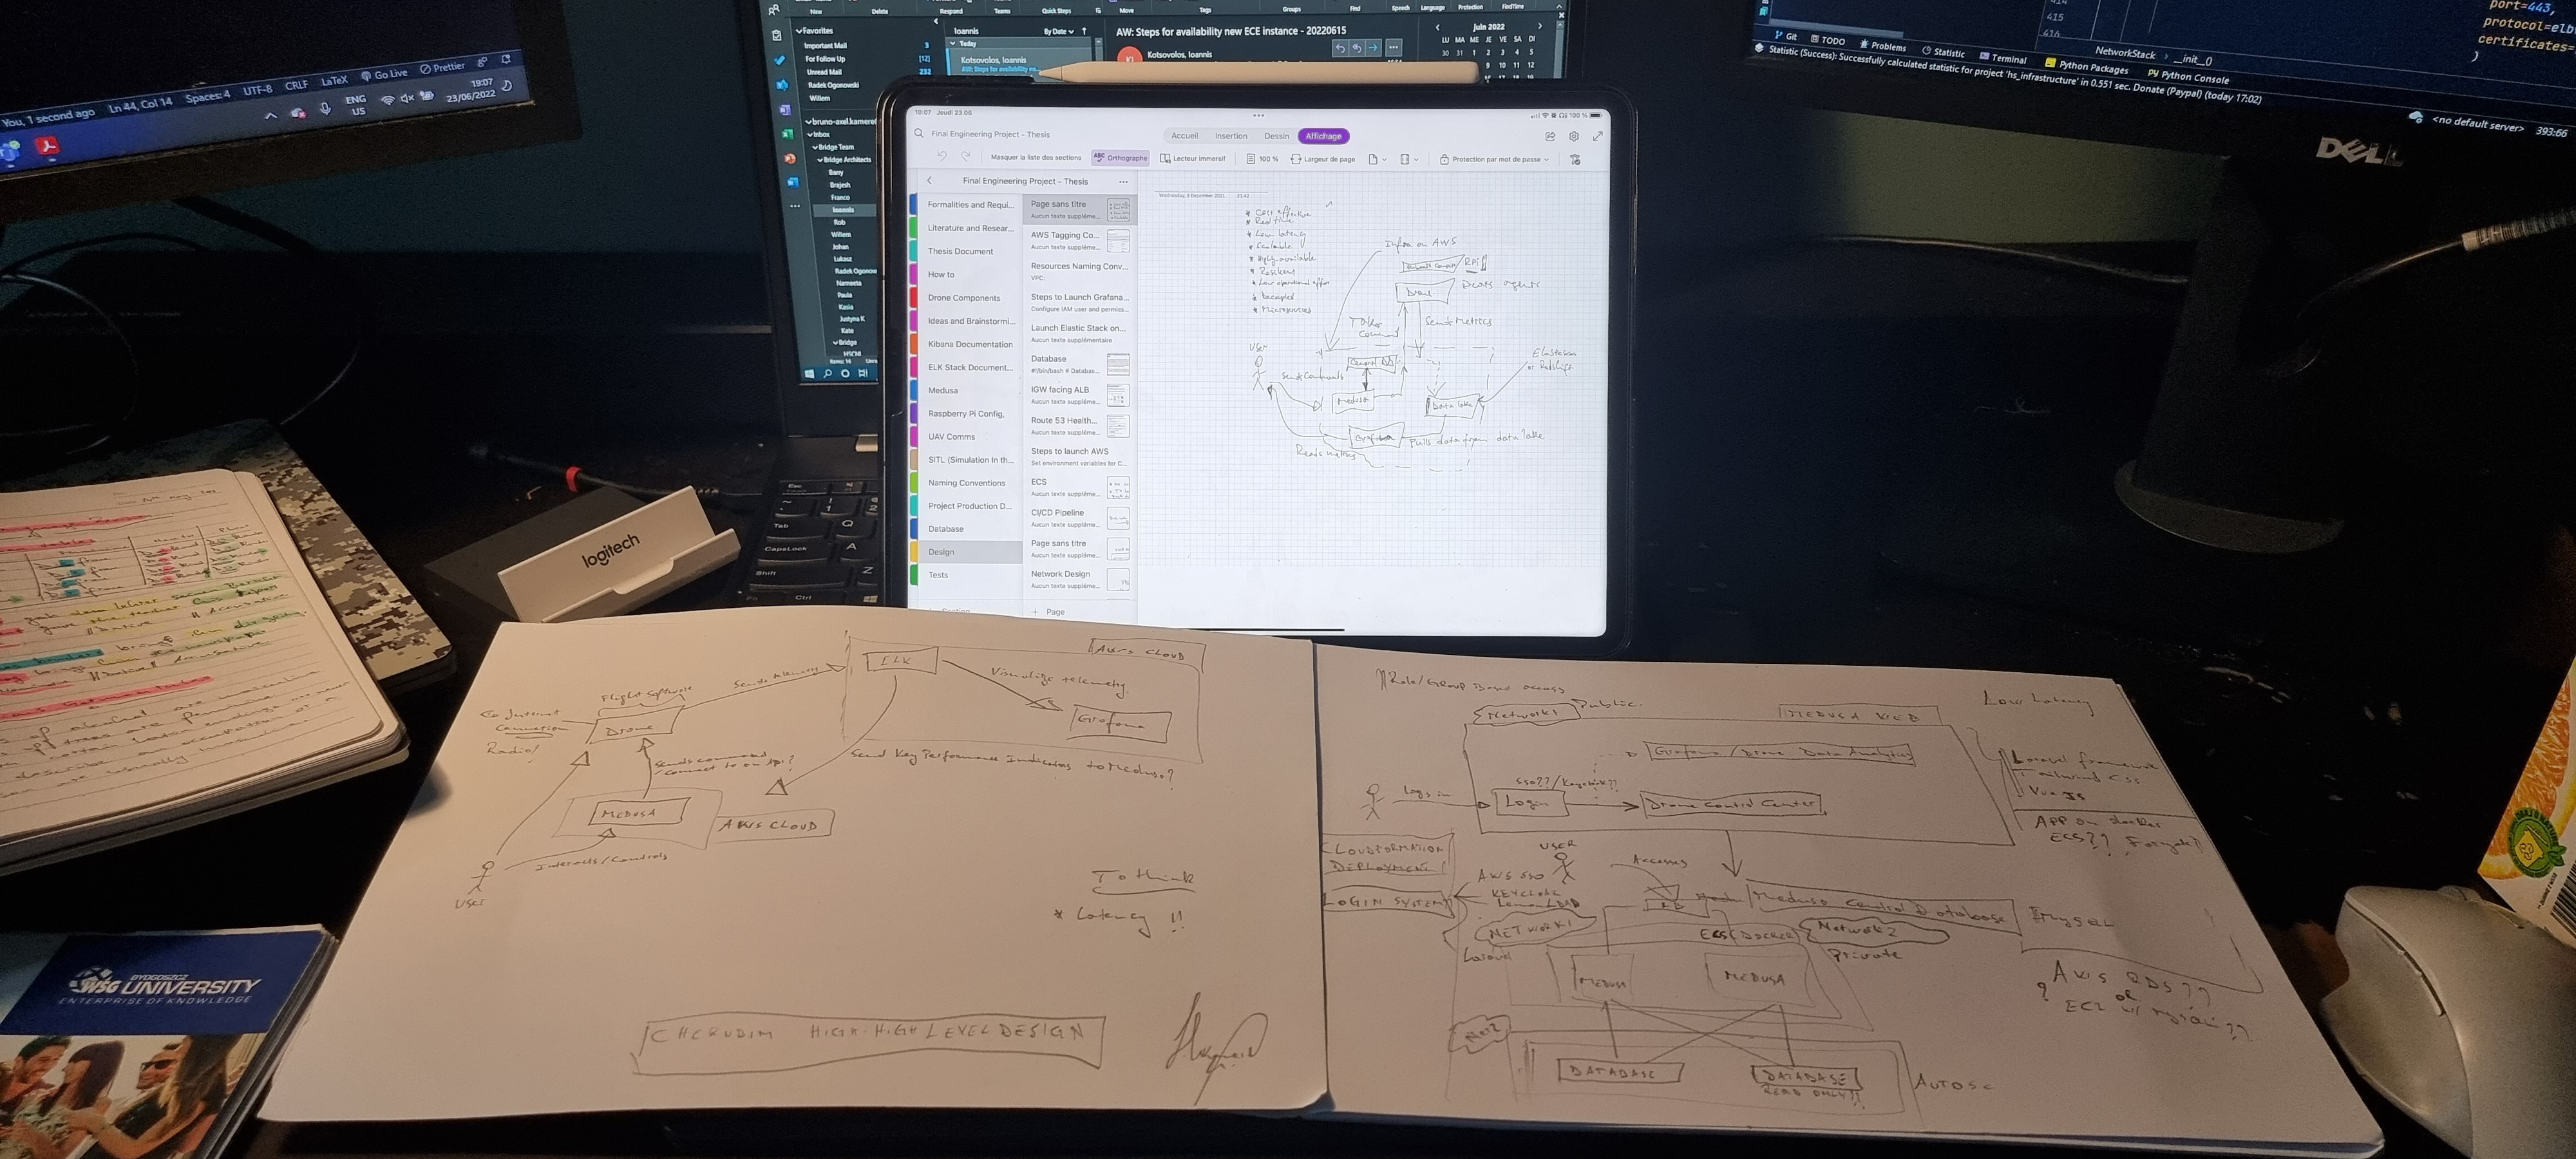
\includegraphics[width=0.9\linewidth]{initial_designs_2.jpg}
    \caption{Initial draft architecture designs.}
    \label{fig:initial-draft-designs}
    \source{Own work.}
\end{figure}

As the design started being built to reality, it was evident that deploying the whole AWS infrastructure manually from the AWS console, see figure <REFERENCE THE AWS CONSOLE>, was going to be a time consuming, inefficient activity. And this also contracdited the initial idea of building an agile infrastructure that can easily be redeployed in case changes are needed. That is where the thought to build the infrastructure as code using some sort of infrastructure as code (IaC) tool came in. Since the cloud provider of choice was AWS, the best tool for the task was with no doubt the AWS cloud development kit <CITE AWS CDK>.

After the AWS infrastructure was built, the next step was the UAV. The outstanding questions here were:

\begin{itemize}
    \item How is the UAV going to be built?
    \item What is going to be the size?
    \item What is going to be the UAV type? Quadcopter? Fixed wing?
    \item How is the UAV going to be programmed? What programming language should be used?
    \item How is the UAV going to communicate with the rest of the system on AWS?
\end{itemize}

The above questions drove the next development stage. The drone type and size of choice were a small quadcopter. The initial idea was to build an actual quadcopter, therefore the below parts were purchased to build the quadcopter:

\begin{itemize}
    \item Readytosky S500 quadcopter frame with built-in PCB.
    \item Pixhawk 2.4.8 flight controller with 4GB of onboard SD card storage.
    \item Raspberry Pi 4 model B with 4GB of onboard SD card storage.
    \item Readytosky M8N GPS module built-in compass with GPS antenna mount.
    \item 4 pieces of A2212 1000KV brushless motors.
    \item 4 pieces of 2-6S 30 amps Electronic speed controllers.
    \item 2 pairs of 1238 carbon fiber propellers.
\end{itemize}

<INSERT AN IMAGE OF THE ABOVE PARTS>

As the development of the quadcopter went on, it became obvious that this approach was not the best way to go, especially for a proof-of-concept (POC) solution mainly due to how costly it was becoming. At somepoint the wire connectors were even insufficient, and it would take too long to order new ones online. The idea to build the actual physical quadcopter was then put on-hold, and it was decided to rather use simulation tools to simulate the actual quadcopter. Section \ref{sec:software-in-the-loop} elaborates more on how the simulation was set up.

<REVEW THIS SECTION>

\section{Solution description}
<ATTACH THE HLD AND DESCRIBE EVERY CONNECTION>

\subsection{AWS cloud development kit setup}
As mentioned in the previous chapters, the designed AWS infrastructure was deployed as code using AWS cloud development kit (AWS CDK). AWS CDK allows developers to build AWS infrastructures in an agile manner by using normal programming languages. This allows developers to take advantage of programming idioms like loops, variables, conditionals and inheritance to build robust AWS infrastructures. This also means that software engineering practices like source control, testing and code reviews can be used since the infrastructure is basically standard code. Currently AWS CDK supports Python, Javascript, C\#, Go, and Typescript programming languages.

A typical AWS CDK project is made up of 3 components, namely:

\begin{itemize}
    \item an app. This is the overall set of everything. An AWS CDK project is basically called an AWS CDK app. This comprises of constructs.
    \item constructs. These represent components that make an AWS infrastructure. They can be an AWS simple storage service (S3), an elastic cloud compute (EC2), an application load balancer (ALB) \textit{et cetera}. AWS has a comprehensive site that shows all the available AWS and community constructs\cite{awsconstructhub}.
    \item stacks. These are the unit of deployment in AWS CDK. A stack represents all AWS resources defined within the same scope.
\end{itemize}

Figure \ref{fig:aws-cdk-app-structure} shows how an AWS CDK app is structured.

\begin{figure}[H]
    \centering 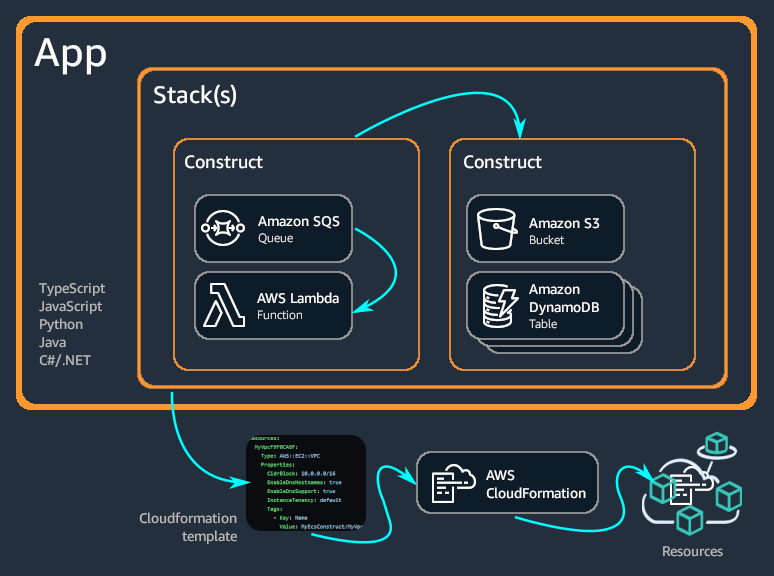
\includegraphics[width=0.9\linewidth]{aws_cdk_workflow.png}
    \caption{AWS CDK app structure.}
    \label{fig:aws-cdk-app-structure}
    \source{AWS CDK documentation\cite{awscdkdocumentation}.}
\end{figure}

\subsection*{Build}

To start building the AWS infrastructure with AWS CDK, the AWS command line interface (CLI) needs to first be set up. To install the AWS CLI on Windows, run the following command \mintinline[breaklines, breakanywhere]{bash}{msiexec.exe /i https://awscli.amazonaws.com/AWSCLIV2.msi}. This allows to interact with AWS via the CLI.

Once the AWS CLI is installed, type the command \mintinline[breaklines, breakanywhere]{bash}{aws configure} to configure credentials to AWS. The console will ask for the AWS access key ID, the AWS secret access key, the default region name and the default output format as shown in figure \ref{fig:aws-configure-output}.

\begin{figure}[H]
    \centering 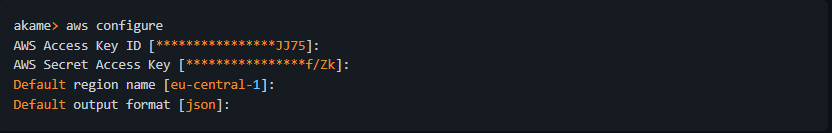
\includegraphics[width=0.9\linewidth]{aws_configure_output.png}
    \caption{AWS configure CLI output.}
    \label{fig:aws-configure-output}
    \source{Own work.}
\end{figure}

The next step is to then install AWS CDK from node package manager (NPM) with \mintinline[breaklines, breakanywhere]{bash}{npm install -g aws-cdk}. This will download and install the latest aws-cdk version on the local workstation. The "-g" flag makes the package available globally on the workstation.

Next, get the account number from the AWS CLI using the AWS security token service (STS) and the region name from AWS CLI configuration by executing the commands below.

\mintinline[breaklines, breakanywhere]{bash}{aws sts get-caller-identity}, to get the account number.

\mintinline[breaklines, breakanywhere]{bash}{aws configure get region}, to get the region name.

\begin{figure}[H]
    \centering 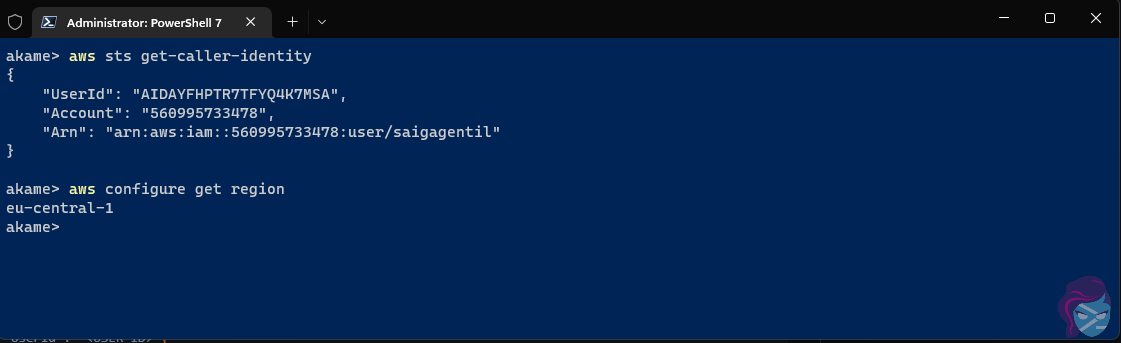
\includegraphics[width=0.9\linewidth]{cdk_pre_bootstrap.png}
    \caption{AWS STS and configure commands output.}
    \label{fig:aws-account-numbre-region}
    \source{Own work.}
\end{figure}

With the account number and the region name, AWS CDK can be bootstrapped now. Bootstrapping in AWS refers to the process of creating assets (local files, directories, docker image,...) that need to be deployed with the stack. These assets are deployed to an AWS S3 bucket for AWS CloudFormation to use them during stack deployment. Execute command \mintinline[breaklines, breakanywhere]{bash}{cdk bootstrap aws://560995733478/eu-central-1} to bootstrap AWS CDK.

Once all the above steps are completed, a CDK app can now be created. First create a directory for the app and move into the directory, \mintinline[breaklines, breakanywhere]{bash}{mkdir hs_infrastructure} then \mintinline[breaklines, breakanywhere]{bash}{cd hs_infrastructure},then run the command \mintinline[breaklines, breakanywhere]{bash}{cdk init app --language python} to initialize a Python AWS CDK app. After that, activate the Python virtual environment with \mintinline[breaklines, breakanywhere]{bash}{source .venv/Scripts/activate} and install the core AWS CDK plugins with \mintinline[breaklines, breakanywhere]{bash}{python -m pip install -r requirements.txt}.

This will generate a couple of starting files in the app directory. Also if Git is installed on the workstation the app will be initialized as a Git repository that can be versioned and later be pushed to a Git remote repository like Github.

\subsection*{Deploy}

After completing the previous steps, we have an app with a default stack but with no resources defined in it. The next step is to write code that defines stacks that make the AWS infrastructure. In the proposed solution, multiple stacks were created, figure \ref{fig:aws-stacks} shows the stacks that make the proposed solution.

\begin{figure}[H]
    \centering 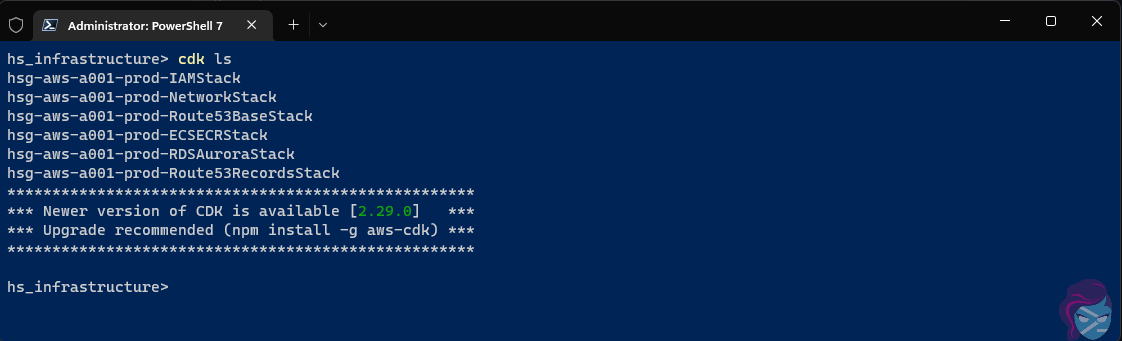
\includegraphics[width=0.9\linewidth]{cdk_ls.png}
    \caption{Proposed solution AWS stacks.}
    \label{fig:aws-stacks}
    \source{Own work.}
\end{figure}

Each of the stacks defines several services needed to build the whole overall infrastructure.
\begin{itemize}
    \item hsg-aws-a001-prod-IAMStack: Creates IAM user needed by the AWS elastic container service (ECS) and elastic container registry (ECR).
    \item hsg-aws-a001-prod-NetworkStack: Sets up the overall AWS infrastructure networking. Subnets, firewall rules, \textit{et cetera}. This is the longest stack in terms of lines of code, because it is made up of approximately 480 lines of code.
    \item hsg-aws-a001-prod-Route53BaseStack: This creates a hosted zone for the domain helloskygroup.com as well as a wildcard SSL certificate for the domain.
    \item hsg-aws-a001-prod-ECSECRStack: This spins up docker containers hosting the web application in the AWS ECS Fargate service. Fargate was used since it is a serverless service. A serverless service is a service that offloads the responsibility from developers to managed the actual physical servers hosting the deployed resources.
    \item hsg-aws-a001-prod-RDSAuroraStack: This deploys a MySQL database in the AWS relational database service (RDS).
    \item hsg-aws-a001-prod-Route53RecordsStack: This adds DNS records in the hosted zone created in the 'hsg-aws-a001-prod-Route53BaseStack' stack.
\end{itemize}

Once each stack is developed, the next step is to deploy it to AWS. Snippet \ref{code:hs_infrastructure_app_snippet_1} shows the \mintinline[breaklines, breakanywhere]{python}{main.py} code that basically imports all the created tasks in the AWS app and executes them. From there, the command \mintinline[breaklines, breakanywhere]{bash}{cdk deploy -all} needs to be executed from the root directory to deploy the resources and stacks defined in the app. Figure \ref{fig:aws-cdk-app-lifecycle} shows the full lifecycle of an AWS CDK app.

\begin{figure}[H]
    \centering 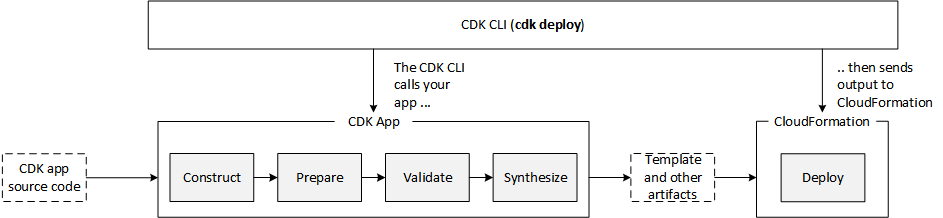
\includegraphics[width=0.9\linewidth]{aws_cdk_app_lifecycle.png}
    \caption{AWS CDK app lifecycle.}
    \label{fig:aws-cdk-app-lifecycle}
    \source{AWS documentation\cite{awscdkdocumentationapps}.}
\end{figure}

\begin{center}
    \captionsetup{type=listing}
    \inputminted[
        frame=single,
        framesep=2mm,
        baselinestretch=1.2,
        fontsize=\footnotesize,
        breaklines,
        breakanywhere,
        linenos
    ]{python}{config/code/47c895ea0838ad6366c2b0e53bb8c331/hs_infrastructure_app_snippet_1.py}
    \captionof{listing}{AWS CDK app.py snippet.}
    \label{code:hs_infrastructure_app_snippet_1}
\end{center}


\section{AWS Network access and security}
One of the challenges with implementing a networked system, especially on cloud platforms like AWS, is ensuring that traffic flows in the expected way with proper security in place. The proposed solution, being a networked solution involving communications to and from various applications, has a rigorous network design. Figure <REFERENCE TO THE NETWORK DESIGN IMAGE> shows how network within the proposed AWS infrastructure was designed.

AWS has a concept of Virtual Private Cloud also known as VPC, which is simply an isolated private network that can be broken down into various subnets depending on the architecture. The proposed solution has one VPC broken down into three subnets; public, private and isolated-private subnets for each availability zone.

\subsection{Public subnet}
\label{public-subnet}
The public subnet in this proposed solution does not contain any resources, except a Network Address Translation or NAT gateway that is used by resources in the private subnet to access the internet. Table \ref{table:public-subnet-inbound} and \ref{table:public-subnet-outbound} show the inbound and outbound traffic rules respectively configured on the public subnet network access control list or NACL.

\begin{table}[H]
    \centering
    \begin{tabular}{|c|c|c|c|c|c|}
        \hline
        \multicolumn{6}{|c|}{Inbound traffic}                               \\
        \hline
        Rule & Type        & Protocol & Port range & Source    & Allow/Deny \\
        \hline
        100  & HTTP (80)   & TCP (6)  & 80         & 0.0.0.0/0 & Allow      \\
        \hline
        110  & HTTPS (443) & TCP (6)  & 443        & 0.0.0.0/0 & Allow      \\
        \hline
        120  & Custom TCP  & TCP (6)  & 1024-65535 & 0.0.0.0/0 & Allow      \\
        \hline
        *    & All IPV4    & All      & All        & 0.0.0.0/0 & Deny       \\
        \hline
    \end{tabular}
    \caption{Public subnet NACL inbound traffic rules}
    \label{table:public-subnet-inbound}
\end{table}

\begin{itemize}
    \item \textbf{Rule 100:} Allows inbound HTTP traffic on port 80 towards any IPv4 address on the internet.
    \item \textbf{Rule 110:} Allows inbound HTTPS traffic on port 443 towards any IPv4 address on the internet.
    \item \textbf{Rule 120:} Allows returning TCP traffic from the internet responding to requests from the subnet. The specified port ranges are ephemeral ports as defined by the Internet Assigned Number Authority or IANA and Internet Engineering Task Force or IETF in their Request for Comments or RFC 6056 document \cite{rfc6056}.
    \item \textbf{Rule *:} Block every other non previously evaluated IPv4 traffic.
\end{itemize}

\begin{table}[H]
    \centering
    \begin{tabular}{|c|c|c|c|c|c|}
        \hline
        \multicolumn{6}{|c|}{Outbound traffic}                                \\
        \hline
        Rule & Type        & Protocol & Port range & Destination & Allow/Deny \\
        \hline
        100  & HTTP (80)   & TCP (6)  & 80         & 0.0.0.0/0   & Allow      \\
        \hline
        110  & HTTPS (443) & TCP (6)  & 443        & 0.0.0.0/0   & Allow      \\
        \hline
        120  & Custom TCP  & TCP (6)  & 1024-65535 & 0.0.0.0/0   & Allow      \\
        \hline
        *    & All IPV4    & All      & All        & 0.0.0.0/0   & Deny       \\
        \hline
    \end{tabular}
    \caption{Public subnet NACL outbound traffic rules}
    \label{table:public-subnet-outbound}
\end{table}

The rules explanation are similar to those for inbound traffic in table \ref{table:public-subnet-inbound}, except that instead of inbound it is outbound.

\subsection{Private subnet}
\label{private-subnet}
Most of the infrastructure components are deployed in the private subnet where only specific traffic from the public and isolated-private subnets are allowed in. In this subnet is where the UAV command and control center user interface is deployed, in containers using the AWS Fargate serverless service. The rules for this subnet have to be carefully defined so that;

\begin{itemize}
    \item Fargate services can pull docker images from docker hub public repositories on the internet.
    \item The UAV, and several command and control application services can talk to each other.
\end{itemize}

Table \ref{table:private-subnet-inbound} and \ref{table:private-subnet-outbound} show the inbound and outbound traffic rules respectively configured on the private subnet network access control list or NACL.

\begin{table}[H]
    \centering
    \begin{tabular}{|c|c|c|c|c|c|}
        \hline
        \multicolumn{6}{|c|}{Inbound traffic}                                 \\
        \hline
        Rule & Type        & Protocol & Port range & Source      & Allow/Deny \\
        \hline
        100  & HTTP (80)   & TCP (6)  & 80         & 0.0.0.0/0   & Allow      \\
        \hline
        110  & HTTPS (443) & TCP (6)  & 443        & 0.0.0.0/0   & Allow      \\
        \hline
        120  & Custom TCP  & TCP (6)  & 1024-65535 & 0.0.0.0/0   & Allow      \\
        \hline
        130  & Custom TCP  & TCP (6)  & 3306       & 10.0.4.0/28 & Allow      \\
        \hline
        140  & Custom TCP  & TCP (6)  & 3306       & 10.0.5.0/28 & Allow      \\
        \hline
        *    & All IPV4    & All      & All        & 0.0.0.0/0   & Deny       \\
        \hline
    \end{tabular}
    \caption{Private subnet NACL inbound traffic rules}
    \label{table:private-subnet-inbound}
\end{table}

\begin{itemize}
    \item \textbf{Rule 100:} Allows inbound HTTP traffic on port 80. This is so that the AWS Elastic Container Service or ECS tasks can pull images from the public Dockerhub registry.
    \item \textbf{Rule 110:} Allows inbound HTTPS traffic on port 443.
    \item \textbf{Rule 120:} Allows returning TCP traffic from the internet responding to requests from the subnet.
    \item \textbf{Rule 130 and Rule 140:} Allows inbound traffic on port 3306 from MySQL database running in the AWS Relational Database Service or AWS within the isolated-private subnets of both the Availability Zones.
    \item \textbf{Rule *:} Blocks every other non previously evaluated IPv4 traffic.
\end{itemize}

\begin{table}[H]
    \centering
    \begin{tabular}{|c|c|c|c|c|c|}
        \hline
        \multicolumn{6}{|c|}{Outbound traffic}                                \\
        \hline
        Rule & Type        & Protocol & Port range & Destination & Allow/Deny \\
        \hline
        100  & HTTP (80)   & TCP (6)  & 80         & 0.0.0.0/0   & Allow      \\
        \hline
        110  & HTTPS (443) & TCP (6)  & 443        & 0.0.0.0/0   & Allow      \\
        \hline
        120  & Custom TCP  & TCP (6)  & 1024-65535 & 0.0.0.0/0   & Allow      \\
        \hline
        130  & Custom TCP  & TCP (6)  & 3306       & 10.0.4.0/28 & Allow      \\
        \hline
        140  & Custom TCP  & TCP (6)  & 3306       & 10.0.5.0/28 & Allow      \\
        \hline
        *    & All IPV4    & All      & All        & 0.0.0.0/0   & Deny       \\
        \hline
    \end{tabular}
    \caption{Private subnet NACL outbound traffic rules}
    \label{table:private-subnet-outbound}
\end{table}

\begin{itemize}
    \item \textbf{Rule 100:} Allows outbound HTTP traffic on port 80 towards any IPv4 address.
    \item \textbf{Rule 110:} Allows outbound HTTPS traffic on port 443 towards any IPv4 address.
    \item \textbf{Rule 120:} Allows all outbound response TCP traffic.
    \item \textbf{Rule *:} Blocks every other non previously evaluated IPv4 traffic.
\end{itemize}

<TALK ABOUT SECURITY GROUPS>

\subsection{Isolated-private subnet}
\label{isolated-private-subnet}

The isolated-private subnet hosts the MySQL database running in AWS Relational Database Service. This subnet only talks to the private subnet, and has no direct connection to the internet. This improves the infrastructure security through not exposing the database directly to the internet.

<ADD NETWORK FLOW DESIGNS>

Describe the solution on a higher level. Discuss HLDs.

\section{Software in the loop UAV simulator}
\label{sec:software-in-the-loop}


\section{UAV Communication}
<Talk about Mavlink... and how mavlink is used in the project>

\nomenclature[z-AZ]{AZ}{Availability Zone}
\nomenclature[z-NAT]{NAT}{Network Address Translation}
\nomenclature[z-VPC]{VPC}{Virtual Private Cloud}
\nomenclature[z-HTTP]{HTTP}{Hypertext Transfer Protocol}
\nomenclature[z-HTTPS]{HTTPS}{Hypertext Transfer Protocol Secured}
\nomenclature[z-ECS]{ECS}{Elastic Container Service}
\nomenclature[z-NACL]{NACL}{Network Access Control List}
\nomenclature[z-EC2]{EC2}{Elastic Cloud Compute}
\nomenclature[z-TCP]{TCP}{Transmisison Control Protocol}
\nomenclature[z-RDS]{RDS}{Relational Database Service}
\nomenclature[z-ALB]{ALB}{Application Load Balancer}
\nomenclature[z-RDS]{RDS}{Relational Database Service}
\nomenclature[z-IANA]{IANA}{Internet Assigned Number Authority}
\nomenclature[z-IETF]{IETF}{Internet Engineering Task Force}
\nomenclature[z-RFC]{RFC}{Request for Comments}
\nomenclature[z-PCB]{PCB}{Printed Circuit Board}
\nomenclature[z-SD]{SD (as in SD card)}{Secure Digital}
\nomenclature[z-GPS]{GPS}{Global Positioning System}
\nomenclature[z-S3]{S3 (as in AWS S3)}{Simple Storage Service}
\nomenclature[z-CLI]{CLI}{Command Line Interface}
\nomenclature[z-IAM]{IAM}{Identity Access Management}
\nomenclature[z-ECR]{ECR}{Elastic Container Registry}
